\documentclass[twocolumn]{aastex62}

\usepackage[utf8]{inputenc}
\usepackage{url}
\usepackage{xspace}
\usepackage{natbib}  % Requires natbib.sty, available from http://ads.harvard.edu/pubs/bibtex/astronat/
\usepackage{minted}

\newcommand{\pyspeckit}{\texttt{pyspeckit}\xspace}
\newcommand{\astropy}{\texttt{astropy}\xspace}
\newcommand{\hh}{\ensuremath{\mathrm{H}_2}\xspace}
\newcommand{\ammonia}{\ensuremath{\mathrm{NH}_3}\xspace}
\begin{document}

\title{{\sc{pyspeckit}:} A spectroscopic analysis and plotting package}
%\authorrunning{Ginsburg et al}

\author[0000-0001-6431-9633]{Adam Ginsburg}
%\nraojansky

\author{Vlas Sokolov}
\author{Miguel de Val-Borro}
\author{Allison Youngblood}
\author{Erik Rosolowsky}
\author[0000-0002-3972-1978]{Jaime E. Pineda}
\author[0000-0002-3713-6337]{Brigitta M. Sip\H{o}cz}


\begin{abstract}
\pyspeckit is a tool and library for spectroscopic analysis in Python. We
describe the \pyspeckit package and highlight some of its unique capabilities
such as interactively fitting a model to data, akin to the widely-used
\texttt{splot} function of \texttt{IRAF}. \pyspeckit employs the
Levenberg-Marquardt optimization method via \texttt{mpfit} and \texttt{lmfit},
and important assumptions regarding error estimation are described here.
Wrappers for \texttt{pymc} and \texttt{emcee} are available, as well as a
method to fit lines in spectral cubes. As part of the \astropy affiliated
packages, \pyspeckit is open source and welcomes input and collaboration from
the community.
\end{abstract}


\section{Introduction}
Spectroscopy is an important tool for astronomy. Spectra are represented as
the number of photons, or total energy in photons, arriving over a specified
wavelength (or equivalently, frequency or energy) range. Emission and
absorption lines due to ions, atoms, and molecules bear important information
via their intensity, width, and velocity centroid. These parameters are
typically measured from model fits to the data, such as Gaussians, Lorentzians,
and Voigt profiles. Historically, \texttt{IRAF} has provided the astronomy
community with easy-to-use tools for line fitting, but \texttt{IRAF}
development has mostly ceased in the last several years and is currently only
supported in Python 2.7 by
AstroConda\footnote{http://astroconda.readthedocs.io/en/latest/index.html},
though the PyRAF command language
(\url{https://github.com/spacetelescope/pyraf}) supports both Python 2 and
Python 3 and is still maintained.


\pyspeckit development began in 2009 with a script called `showspec'
in the \texttt{agpy} package hosted on Google Code. It was created and used by
a graduate student to plot and sometimes fit profiles to spectra in python. At the time,
IDL was still more popular than python at most institutes \citep[first evidence
that python had overtaken IDL in popularity among astronomers was presented in
]{Momcheva2015a}, and there were no publicly available and advertised tools for
spectral plotting, fitting, and general manipulation \cite[\texttt{astropysics}
was developed contemporaneously and solved many of the same problems as
\pyspeckit][]{Tollerud2012a}. The \astropy project had its first commit in
2011, so even the basic infrastructure for such analysis was not yet
established.

\pyspeckit's graphical user interface (GUI) features were inspired by IRAF's
\texttt{splot} tool, while the fitting features were inspired in part by \texttt{xspec}
(\url{https://heasarc.gsfc.nasa.gov/xanadu/xspec/}).  Over subsequent years,
\pyspeckit grew by incorporating more sophisticated models  and improving its
internal structure.  The package was moved out of \texttt{agpy} and into its
own repository in 2011, first spending a few years on Bitbucket in a mercurial
repository, then finally moved to GitHub, where it currenly resides, in 2012.

Because \pyspeckit's initial development preceded \astropy, some features
were included that later became redundant with \astropy.  Most notably, \pyspeckit included
a limited system for spectroscopic unit conversion.  In 2015, this system
was completely replaced with \astropy's unit system.  Around the same time,
the Doppler conversion tools (converting from frequency or wavelength to
velocity) that existed in \pyspeckit were pushed upstream into \astropy,
highlighting the mutually beneficial role of \astropy's affiliated
packaged system \citep{Astropy_2018}.  \pyspeckit was finally
accepted as an \astropy affiliated package in 2017.


In this paper we briefly outline \texttt{pyspeckit} architecture and highlight
its key capabilities. In Section \ref{sec:basicstructure}, we  outline the
basic structure of the package.  In Section \ref{sec:gui}, we describe the GUI
system.  In Sections \ref{sec:cubes} and \ref{sec:models}, we outline
\pyspeckit's cube handling capabilities and model library.



\section{Basic structure}
\label{sec:basicstructure}
The central object in \pyspeckit is a \texttt{Spectrum} object, which has
associated \texttt{data} (e.g., flux), \texttt{error}, and \texttt{xarr} (e.g., wavelength,
frequency, energy), the latter of
which represents the spectroscopic axis.  A \texttt{Spectrum} object has
several attributes that are themselves sophisticated classes that can be called
as functions: the \texttt{plotter}, the fitter \texttt{specfit}, and the
continuum fitter \texttt{baseline}\footnote{It is common in radio astronomy to
have wide instrumental residual features in the data that need to be fitted and
removed; this process is called `baseline subtraction'.  In other wavelength
regimes, this would typically be referred to as continuum fitting or continuum
subtraction.  In practical algorithmic terms, fitting a true astrophysical
continuum and a residual instrumental baseline are indistinguishable.}.

There are several important subclasses of \texttt{Spectrum}: \texttt{Spectra}
is a collection of spectra intended to be stitched together (i.e., with
non-overlapping spectral axes), \texttt{ObsBlock} is a collection of spectra
with identical spectral axes intended to be operated on as a group, e.g., to
take an average spectrum, and \texttt{Cube} is a 3D spatial-spatial-spectral
cube.

\subsection{Supported data formats}

\pyspeckit supports a variety of open and proprietary data formats that have
been traditionally used to store spectral data products in astronomy.
We list the currently supported formats here:

\begin{itemize}
    \item ASCII: Reading a one-dimensional spectrum from a text file with an optional
        error column can
	be done using the \texttt{astropy.io.ascii} module in any of its supported
	formats.
    \item FITS: The Flexible Image Transport System \citep[FITS;][]{Wells1981a,Greisen2006a,Pence2010a} format is
	supported in \pyspeckit with \texttt{astropy.io.fits}.  
    FITS spectra are expected to have their spectral axis defined using the WCS
    keywords in the FITS header.  FITS binary tables can also be used.
    %Initially developed
	%by optical astronomers, the FITS standard has incorporated several
	%recommendations for various types of data formats used in the astronomy
	%community into successive updates to the standard---the latest version of the
	%standard being 4.0 from 2016.  
    \item SDFITS: Data files following the Single
	Dish FITS \citep[SDFITS;][]{Garwood2000a} convention for radio astronomy data as
	produced by the Green Bank Telescope are partially supported in \pyspeckit.
	% \authorcomment1{Is it possible to clarify what is not supported?
    % Or up to which version of SDFITS it is working?} No, I don't know the
    % answers to this; it would take some real work to find out.
    \item HDF5: The Hierarchical Data Format (HDF5) file format has been
        designed to store and organize large amounts of data and offers
        significant advantages over FITS\@.  Although not widely used in
        observational astronomy, the pipeline of the Low-Frequency Array
        (LOFAR) radio telescope uses the HDF5 data format to efficiently store
        large data volumes \citep{Alexov2012a}.  If the \texttt{h5py} package
        is installed, \pyspeckit will support read access to files containing
        spectra in the HDF5 format (although there is no specified standard for
        spectra in HDF5, so additional user effort may be required to create
        \pyspeckit Spectrum objects from the extracted HDF5 data).
    \item Finally, \pyspeckit is capable of reading files from some versions of
        the GILDAS Continuum and Line Analysis Single-dish Software format
        \citep[CLASS;][]{Gildas-Team2013a}.  
	% Since the CLASS file specification
        % is incomplete and will remain private for the foreseeable future, much
        % of the data reading in \pyspeckit has been reproduced in an approximate
        % manner.
        %\authorcomment1{Is it possible to mention which range of GILDAS
        %versions have been tested? Is the problem with possible shifts in frequency
        %or in amplitude?}
        %I don't have the tools needed to perform these tests, but perhaps someone
        %else might.
        The CLASS reader is known to be compatible with data files from
        the Arizona Radio Observatory telescopes (12-m and 10-m Submillimeter
        Telescope) and the Atacama Pathfinder Experiment (APEX) radio
        telescope.
\end{itemize}

\subsection{Plotter}
The \texttt{plotter} is a basic plot tool that comprises \pyspeckit's main
graphical user interface.
% [I think a sentence or two of a summary or
% description is needed here - would it be accurate to say something like "that comprises \pyspeckit's
% graphical user interface?]
It is described in more detail in the  GUI section (\S \ref{sec:gui}).

% Should we include code examples of how to do these things? I think examples
% creating a Spectrum, plotting it, interactively fitting, and then
% printing out parinfo on the command line would be neat.

\subsection{Fitter}
\label{sec:fitters}
The fitting tool in \pyspeckit is the \texttt{Spectrum.specfit} object.
This object is a class that is created for every \texttt{Spectrum} object.
The fitter can be used with any of the models included in the model
registry, or a custom model can be created and registered.

To fit a profile to a spectrum, several optimizers are available.  Two
implementations of the Levenberg-Marquardt optimization method
\citep{Levenberg1944a,Marquardt1963a} are provided,
\texttt{mpfit}\footnote{Originally implemented by Craig Markwardt
\url{https://www.physics.wisc.edu/~craigm/idl/fitqa.html} and ported to python
by Mark Rivers and then Sergei Koposov.  The version in pyspeckit has been
updated somewhat from Koposov's version.} and
\texttt{lmfit}\footnote{\url{https://lmfit.github.io/lmfit-py/},
\url{http://dx.doi.org/10.5281/zenodo.11813}}.  Wrappers of
\texttt{pymc}\footnote{\url{https://pymc-devs.github.io/pymc/}} and
\texttt{emcee}\footnote{\url{http://dfm.io/emcee/current/},
\citet{Foreman-Mackey2013a}} are also available, though these tools are better
for parameter error analysis than for optimization.

Once a fit is performed, the results of the fit are accessible through the
\texttt{parinfo} object, which is a dictionary-like structure containing
the parameter values, errors, and other metadata (e.g., information about
whether the parameter is fixed, tied to another parameter, or limited).
Other information about the fit, such as the $\chi^2$ value, are available
as attributes of the \texttt{specfit} object.

\paragraph{Optimal $\chi^2$}
Specfit computes the `optimal' $\chi^2$, which is the $\chi^2$
value computed only over the range where the model contains statistically
significant signal.  By default, the function selects all pixels where
the model value is greater (in absolute value) than the corresponding error.
In principle, this optimal $\chi^2$ may be helpful for obtaining correctly
scaled errors (see Section \ref{sec:parerrest}), though this claim has never
been rigorously tested.

\subsection{Data Selection}
An important feature of the spectral fitter is the ability to select the region
of the spectrum to be fit.  This selection process can either be done manually,
using the \texttt{selectregion} method to set one or more ranges of data to
include in the fit, or interactively using the GUI.  By default, the selected
regions are then highlighted.

\subsection{Continuum Fitting}
The fitting process in \pyspeckit is capable of treating line and continuum
independently or jointly.  If a model includes continuum, e.g., for the case
of a four-parameter Gaussian profile that includes an additive constant, it
can be fitted through the standard \texttt{specfit} fitter.

However, it is common practice to fit the continuum independently prior to
fitting lines.  Such practice is necessary when fitting absorption lines
and practically necessary for heterodyne radio observations where the
continuum is usually poorly measured and corrupted by instrumental effects.  Following radio convention, the \pyspeckit continuum fitting tool is called \texttt{baseline}. This module supports polynomial, spline, and power-law fitting.

\subsection{Error Treatment}
%(Can I refer back to anything here?  like, "Error estimation is an important part of astronomy...")
%(the next two paragraphs may be redundant)

%The basic approach to fit a spectrum is to assign an error to each pixel in the
%\texttt{data} array by providing a value in the \texttt{sp.error} array.  These
%values are assumed to be $1-\sigma$ Gaussian errors on the data.


The \texttt{Spectrum} objects used by \pyspeckit have an attached \texttt{error}
array, which is meant to hold the $1\sigma$ independent Gaussian errors on
each pixel.  While this error representation may be a dramatic
oversimplification of the true errors for almost all instruments (since it ignores correlations between adjacent data), it is also the most
commonly used assumption in astronomical applications.

The \texttt{error} array is used to determine the best-fit parameters and their uncertainties (see
\S \ref{sec:fitters}).  They can be displayed as error bars on individual
pixels or as shaded regions around those pixels using different display modes.

A typical example is given below, where we generate a spectrum and error
array using \texttt{numpy} and \texttt{astropy} tools.

\vspace{2mm}
\begin{minipage}{\linewidth}
\begin{minted}{python}
from astropy import units as u
import numpy as np
import pyspeckit

xaxis = np.linspace(-25, 25)*u.km/u.s
sigma = 3.0*u.km/u.s
data = 5*np.exp(-xaxis**2 /
                (2*sigma**2))*u.Jy
error = np.ones_like(data) * 0.2
sp = pyspeckit.Spectrum(xarr=xaxis,
                        data=data,
                        error=error)

sp.plotter(errstyle='fill')

sp.plotter.savefig("example_fig_1.pdf")
\end{minted}
\end{minipage}

\begin{figure}[!htp]
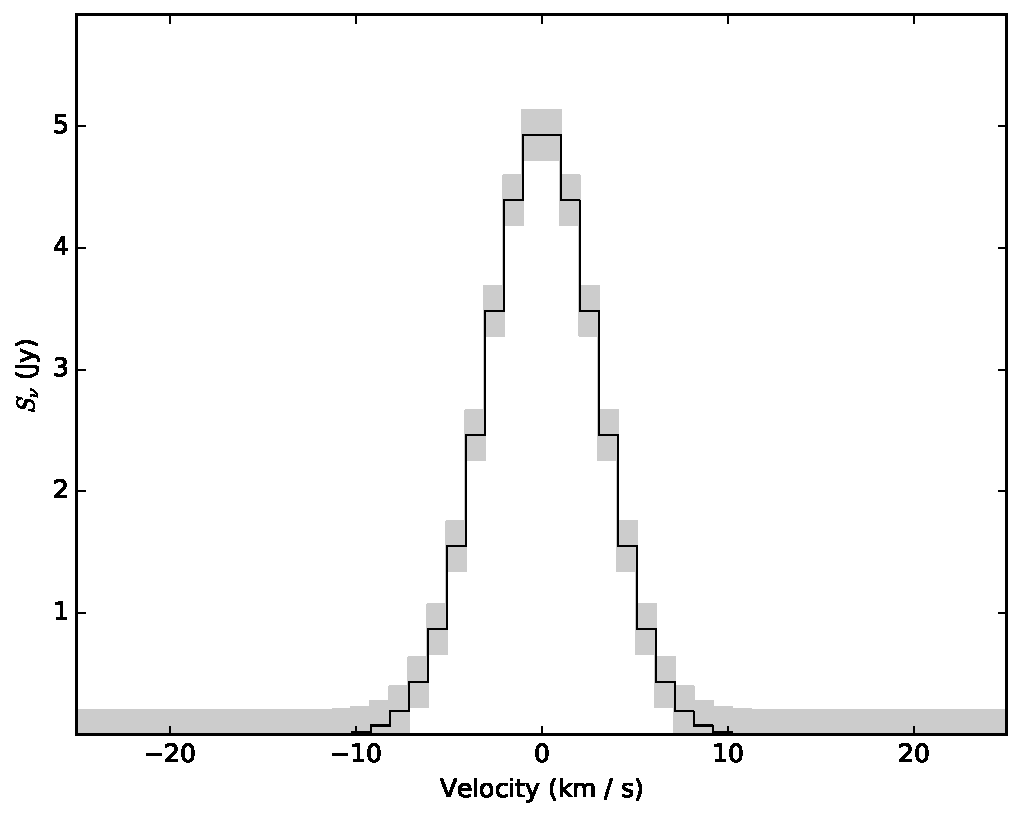
\includegraphics[scale=1,width=3.25in]{example_fig_1.pdf}
\caption{An example plotted spectrum showing the automated unit labeling
and errors.  The errors are shown with the \texttt{`fill'} style
and represent symmetric $1-\sigma$ Gaussian errors.  }
\label{fig:example1}
\end{figure}




\subsubsection{Automatic Error Estimation}
{\color{red} Check that this section is not duplicated elsewhere.}
If a \texttt{Spectrum} is created with no associated errors, \pyspeckit can
automatically estimate the errors from a fit residual. When a fit is initiated
on a \texttt{Spectrum} with no specified errors [I think an example here would be good - just
to make it clear you're talking about calling specfit. We don't yet have a Specfit code
example yet, so this can be worked in with that.],
the errors are set to the default value of 1.0. Thus uniform weighting of the
data is likely to be inaccurate, but will result in the appropriate best-fit
parameters with \emph{incorrect} errors. \textcolor{red}{This is only true if
the data are uniformly weighted but have the incorrect magnitude.  If the data
have different weights, the correct parameters are influenced by the relative
weights.  (Consider an outlier with large vs. small errors).}

In the case where there are clear portions of the spectrum which have no
significant emission, a common approach in spectroscopy is to estimate the
errors from the standard deviation of those signal-free pixels.  This approach
generally assumes the noise is constant across the spectrum.  In the case that
a single signal feature is present in the spectrum, and it can be accurately
modeled, the standard deviation of the residual spectrum from the model fit
will accurately represent the uniform errors. After a fit is performed with
uninitialized errors,
\pyspeckit will automatically replace the errors with the standard deviation of the
residuals; this means that performing a fit on the same data
(without associated errors) twice will result in the same parameter values both
times, but different errors the second time.


\subsubsection{Parameter error estimation}
\label{sec:parerrest}
Parameter errors are adopted from the \texttt{mpfit} or \texttt{lmfit} fit
results.  The Levenberg-Marquardt algorithm finds a local minimum in parameter
space, and one of its returns is the parameter covariance matrix.  This
covariance matrix is not directly the covariance of the parameters, and must be
rescaled to deliver an approximate error.

The standard rescaling is to multiply the covariance by the sum of the squared
errors divided by the degree of freedom of the fit, usually referred to
as $\chi^2/N$.  The number of degrees of freedom is assumed to be equal to the
number of free parameters, e.g., for a one-dimensional Gaussian, there would be
three: the amplitude, width, and center.  This approach implicitly assumes that
the
model describes the data well and is an optimal fit.  It also assumes that
the model is linear with all of the parameters, at least in the region immediately
surrounding the optimal fit.  These requirements are frequently not satisfied;
see \citet{Andrae2010a} and \citet{Andrae2010b} for details.
We show a demonstration of this approximation process in Appendix \ref{appendix:parerrest}
for the case of a simple Gaussian line profile.


% {\color{red} this is redundant with the above}
% One convenience provided by \pyspeckit is also a potential `gotcha': if no
% error is provided, the first time a spectrum is fit, the error will be
% automatically set by computing the standard deviation of the fit residuals.
% Fitting the same spectrum twice may therefore result in different parameter
% errors, but it should never change the fitted parameter values.


\section{Graphical Design}
\label{sec:gui}
\subsection{GUI development}
Many astronomers are familiar with IRAF's \texttt{splot} tool, which is useful
for fitting Gaussian profiles to spectral lines.  It uses keyboard interaction
to specify the fitting region and guesses for fitting the line profile, but for
most use-cases, these parameters could \emph{only} be accessed through the GUI.

The fitting GUI in \texttt{pyspeckit} was built to match \texttt{splot}'s
functionality but with additional means of interacting with the fitter.  In
\texttt{splot}, reproducing any given fit is challenging, since subtle changes
in the cursor position (i.e., the input guess) can significantly change the fit
result.  In \pyspeckit, it is possible to record the results of fits
programmatically and re-fit using those same results.

The GUI was built using \texttt{matplotlib}'s canvas interaction tools.  These
tools are limited to the GUI capabilities that are compatible with all platforms
(e.g., Qt, Tk, Gtk) and therefore exclude some of the more sophisticated fitting
tools found in other software \citep[e.g., \texttt{glue}][]{Beaumont2014b}.

\subsection{Plotting}
Plotting in \pyspeckit is designed to provide a short path to
publication-quality figures.  The default plotting mode uses histogram-style
line plots\added{, which follows the radio and inteferometric standard,} and
labels axes with \LaTeX-formatted versions of units.

When the plotter is active and a model is fit, the model parameters are
displayed with \LaTeX~formatting.  The errors on the parameters, if available,
are also shown, and these uncertainties are used to decide on the number of
significant figures to display.

% \section{\astropy integration}
% Development of \pyspeckit began several years before \astropy began.  Several
% features were therefore implemented that were later replaced by similar
% \astropy features, in particular the unit system.  Unit conversions in
% \pyspeckit are done entirely using the \astropy system since \pyspeckit v0.1.16
% released in May 2015.

\section{Models}
\label{sec:models}
Many of \pyspeckit's internal functions are likely to replaced by the \astropy\
\texttt{specutils} package in the future.  However, the rich suite modeling in
\pyspeckit is likely to remain useful indefinitely.  This model library
includes some of the most useful general spectral model functions (e.g.,
Gaussian, Lorentzian, and Voigt profiles) and a wide range of specific model
types (e.g., ammonia and formaldehyde hyperfine models, the \hh rotational
ladder, and recombination line models).

In radio and millimeter astronomy, there are several molecular line groups that
consist of several Gaussian profiles separated by a fixed frequency offset.
These hyperfine line groups are often unique probes of physical parameters
because these different features have different, known relative optical depths.
In this case, the measured relative amplitudes of these different features
allow the optical depth to be measured from a single spectrum.  \pyspeckit
provides the \texttt{hyperfine} model class to handle this class of molecular
line transitions, and it includes
several molecular species implementations (HCN, N$_2$H$^+$, NH$_3$,
H$_2$CO). Models can customizable and examples of registering a new or modified
model in \pyspeckit are included in the online documentation.
{\color{red}
TODO: ADD MODEL TABLE, maybe add demo of custom model?  That might be in the
docs already...
If this is the beefiest part of pyspeckit, we should include a table
listing the models and potentially an example for how to customize a model?}
\authorcomment1{I (JEP) agree, it would be really useful to include the list of models
already included, and which ones could be used as templates for different types.}


\section{Cubes}
\label{sec:cubes}
Spectral cubes are growing more important in radio astronomy since they are the
natural data products produced by interferometers like ALMA and the JVLA.
Optical and infrared data cubes are also becoming
more common from integral field units (IFUs) like MUSE on
the VLT, OSIRIS on Keck, NIFS on Gemini, and NIRSpec and MIRI on JWST.

While many cube operations are handled well by \texttt{numpy}-based packages
like \texttt{spectral-cube}\footnote{\url{spectral-cube.readthedocs.io}},
it is sometimes desirable to fit a profile to each spectrum
in a cube.  The \texttt{Cube.fiteach} method is a tool for automated line
fitting that includes parallelization of the fit. Implementation examples can be
found in the online documentation.
This tool  has  seen significant use in
custom made survey pipelines,
\citep[e.g.][\url{https://github.com/GBTAmmoniaSurvey/GAS}]{Friesen2017-GAS},
papers and it has been incorporated into other tools (e.g.,
\texttt{multicube}\footnote{\url{https://github.com/vlas-sokolov/multicube}}).


\section{Summary}
\texttt{pyspeckit} is a versatile tool for spectroscopic analysis in python and
is one of the \astropy affiliated packages. \pyspeckit can interactively fit a
model to a spectrum using the Levenberg-Marquardt optimization method via
\texttt{mpfit} and \texttt{lmfit}, and wrappers for \texttt{pymc} and
\texttt{emcee} are also available.  There is also the option to fit a model to
the many spectra in a spectral cube. We have described \pyspeckit's methods of
error estimation for spectra with and without user-provided errors. \pyspeckit
has a library of models including Gaussian, Lorentzian, Voigt, and others for
specific molecular species; user-created models can also be used with
\pyspeckit.

\section{Final Note}
This paper was collaboratively written using GitHub as a platform for
discussion.  Its version history and records of some discussions about its
content can be found at \url{https://github.com/pyspeckit/paper1}.

\input{solobib}


\appendix
\section{Parameter Error Estimation for a simple 1D Gaussian profile}
\label{appendix:parerrest}
As discussed in Section \ref{sec:parerrest}, parameter errors are estimated in
\pyspeckit by the underlying \texttt{lmfit} or \texttt{mpfit} tools using the
approximation that the reduced chi-squared is unity, $\chi^2/n=1$.  We
demonstrate here that, for a simple one-dimensional Gaussian profile, this
approximation results in a reasonable, but not perfect, recovery of the
underlying parameter errors.

In Figure \ref{fig:synthspecdemo}, we show a synthetic spectrum with uniform
Gaussian random noise and perfectly-measured uncorrelated data errors.
The fitted model is a one-dimensional Gaussian profile with free parameters
amplitude, center, and width.  The fit results are given in the figure.

To produce a good error estimate under the $\chi^2/n=1$ approximation, the error
distribution must be Gaussian, the model must be
linear in all parameters, and the model must be the correct underlying model
\citep{Andrae2010b}.

Figure \ref{fig:parerrestdemo} shows the $\chi^2$ values in parameter space
surrounding the best-fit value.  Along the diagonal, we show the $\chi^2$
values varying a single parameter while holding the other two parameters fixed,
i.e., it is the marginal distribution for the free parameter.  The vertical
dashed lines show the estimated $1\sigma$ errors from the optimizer, while the
horizontal dashed lines show the value $\Delta\chi^2=1$, which corresponds to
the 68\% confidence interval for that parameter.  If the $\chi^2/n=1$
approximation were perfect, the dashed lines would intersect with the solid
lines.  For the centroid[or just pick a common term to use - center/shift/centroid]
parameter, the fit is nearly perfect, while for the
amplitude and width, it is not.

Off of the diagonal of Figure \ref{fig:parerrestdemo}, we show the
two-dimensional marginal distributions in which we have held the third
parameter, the one not labeled, fixed.  Contours are shown at
$\Delta\chi^2=2.3,6.2,11.8$, corresponding to 68\%, 95\%, and 99.5\%
($1\sigma$, $2\sigma$, and $3\sigma$ for a Gaussian) confidence regions.  The
vertical and horizontal dashed lines show the estimates from the $\chi^2/n=1$
approximation.
The shift vs amplitude and shift vs width diagrams both show very good matches.
However, the width vs amplitude plot indicates that the single-parameter
errorbars underestimate the true errors because these parameters are
significantly correlated.  This information is captured in the covariance
matrix that is used to compute the single-parameter errors, as it has
significant values in the off-diagonal parts of the matrix.  More broadly, this
approach for estimating parameter uncertainties also relies on the analysis
problem fulfilling the conditions for least-squares fitting, namely that the
dependent variables are perfectly known and that the model would be the correct
representation of perfectly known data.

The source code for this example can be found in the \pyspeckit github
repository in \texttt{examples/synthetic\_spectrum\_example\_witherrorestimates.py}.

\begin{figure*}[!htp]
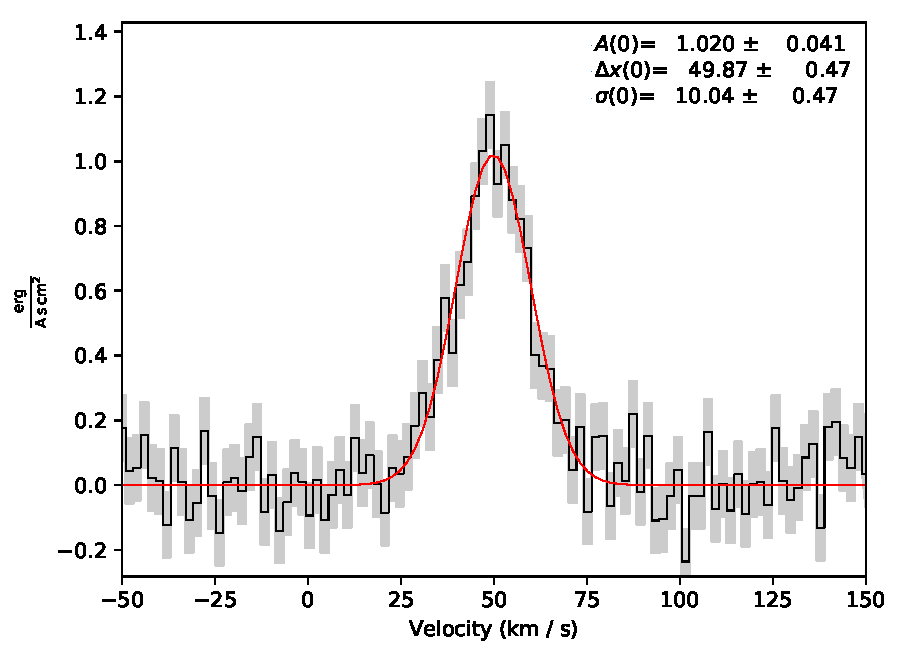
\includegraphics[scale=1,width=7in]{oned_gaussfit_example.pdf}
\caption{One-dimensional Gaussian profile fit to a synthetic spectrum.
The parameter values and errors are shown in the upper right.  The number of
significant figures displayed in both the value and the error is automatically
set to one digit more than the last significant digit in the error.}
\label{fig:synthspecdemo}
\end{figure*}


\begin{figure*}[!htp]
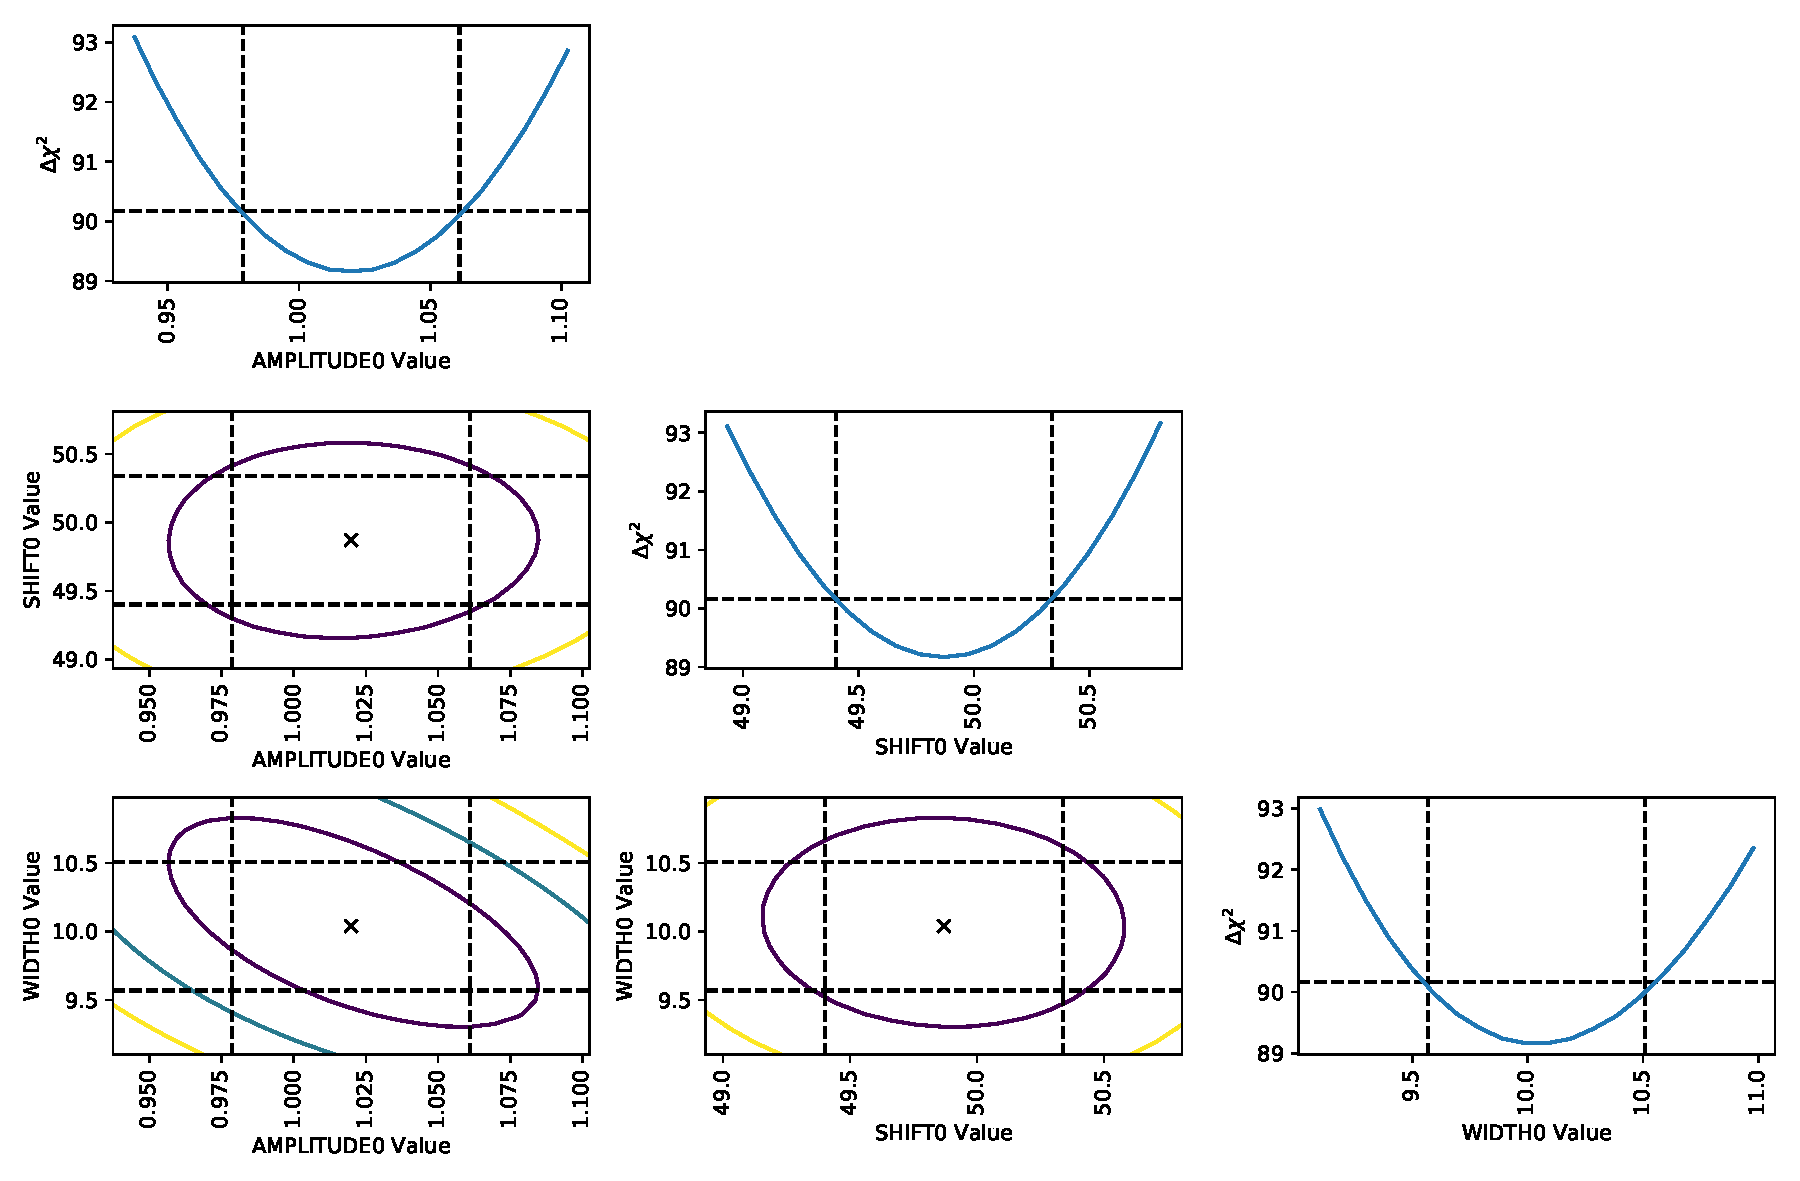
\includegraphics[scale=1,width=7in]{error_estimate_demonstration.pdf}
\caption{Error estimate figure.
In all panels, the vertical
dashed lines show the estimated $1\sigma$ errors from the optimizer, while the
horizontal dashed lines show the value $\Delta\chi^2=1$, which corresponds to
the 68\% confidence interval for that parameter.
In the off-diagonal panels, contours are shown at $\Delta\chi^2=2.3,6.2,11.8$,
corresponding to 68\%, 95\%, and 99.5\% ($1\sigma$, $2\sigma$, and $3\sigma$
for a Gaussian) confidence regions.
See Appendix \ref{appendix:parerrest} for details and interpretation.}
\label{fig:parerrestdemo}
\end{figure*}


\section{Parameter Error Estimation for Ammonia}
\label{appendix:parerrestammonia}
In Section \ref{appendix:parerrest}, we showed the parameter estimation results
in the case of a modeled 1-dimensional Gaussian.  One of the most commonly used
models in \pyspeckit is the ammonia (\ammonia) hyperfine model, which has several
additional emission lines and several parameters governing those lines.

The ammonia inversion transitions are notable for having spectrally resolved
hyperfine components, the relative weights of which are governed by quantum
mechanics \citep{mangum15}. The existence of these additional components often
allows for direct estimates of the optical depth of the central line, which is
optically thicker than the other components, thereby making column density
estimates straightforward when compared to other molecular species.

The model for these lines is more complicated than that for a single Gaussian.
The model must include a simplified version of the radiative transfer equation
and must simultaneously produce the predicted emission of several lines.
Additionally, there are several approximations that are convenient to use
in different circumstances, so \pyspeckit implements several different
variants of the \ammonia model.

In this section, we show parameter estimates analogous to those in Section
\ref{appendix:parerrest}.
We examine a case where the fitted lines are in local
thermodynamic equilibrium (LTE), such that the ratios of the $(J,K)=(1,1)$
to $(2,2)$ line is governed by the rotational temperature $T_\mathrm{R}$ but
the individual lines both have $T_{\mathrm{ex}}=T_{\mathrm{R}}$.
% Second, a case where the fitted lines are not
% in LTE, such that $T_{ex,1-1} \neq T_{ex,2-2}$ and $T_{ex} < T_{R}$; in this case,
% we have adopted these values from a RADEX large velocity gradient model
% \citep{van-der-Tak2007a}.

The free parameters in the ammonia model are the rotational temperature,
$T_{\mathrm{R}}$, which governs the relative populations of the rotational
states, the excitation temperature $T_{\mathrm{ex}}$, which governs the
relative populations of the two levels within a single inversion transition,
the column density, $N(\ammonia)$, which specifies the total column density of
\ammonia integrated over all states (note that this parameter enters the model
as $10^N$, i.e., we optimize the log of the column density), the line-of-sight
velocity $v_\mathrm{LoS}$, the line width $\sigma_v$, and the ortho-to-para
ratio parameterized as the fraction of ortho-\ammonia $F_{ortho}$.  In the
examples below, we fix $F_{ortho}=0$ and treat only para-\ammonia lines.


The fit results from the first case are shown in Figures
\ref{fig:nh3synthspecdemo} and \ref{fig:nh3parerrestdemo}.  The fit recovers
the input parameters, but reveals one of the important caveats when using any
optimization algorithm: in some models, parameters are degenerate, and
therefore using the diagonal of the covariance matrix to estimate the variance
can result in incorrect error estimates.  While the errors on most parameters
appear reasonable, there is a very large error on the excitation temperature
$T_{\mathrm{ex}}$, which is driven by the degeneracy of $T_{\mathrm{ex}}$ with
$N_\mathrm{tot}$.  The asymmetry of the error on $T_{\mathrm{ex}}$ is apparent
in Figure \ref{fig:nh3parerrestdemo}, but it is not captured by the optimizer's
reported error results; the asymmetry occurs because $T_{ex}$ is in the
exponent in the model equations.

In such situations, it can be beneficial to measure the parameter errors
in different ways.  Using the \texttt{emcee} and \texttt{pymc} wrappers
can help do this.  Examples of how to use these Monte Carlo samplers
to acquire better parameter errors once an optimization has already
been performed are available in the online documentation:
see \url{http://pyspeckit.readthedocs.io/en/latest/example_pymc.html}.

More sophisticated examples, including fitting of a non-LTE ammonia spectrum
in which $T_{\mathrm{ex}} < T_{R}$, are available in the example directory
of \pyspeckit (\url{https://github.com/pyspeckit/pyspeckit/tree/master/examples}),
specifically
\url{https://github.com/pyspeckit/pyspeckit/tree/master/examples/synthetic_LTE_ammonia_spectrum_example_witherrorestimates.py}
and
\url{https://github.com/pyspeckit/pyspeckit/tree/master/examples/synthetic_nLTE_ammonia_spectrum_example_witherrorestimates.py}.
These examples also include demonstrations of how to force the optimizer to
ignore nonphysical values.


\begin{figure*}[!htp]
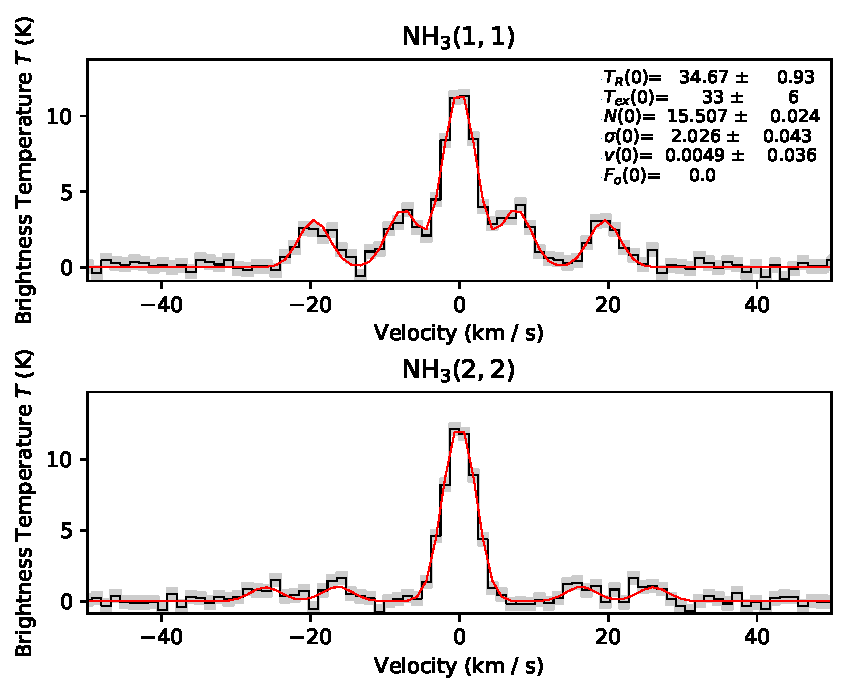
\includegraphics[scale=1,width=7in]{oned_ammonia_LTE_fit_example.pdf}
\caption{Ammonia model profile fit to a synthetic spectrum.
The parameter values and errors are shown in the upper right.  The associated
error estimate triangle diagram is shown in Figure \ref{fig:nh3parerrestdemo}.
The correct parameters are $T_{\mathrm{R}}=T_{\mathrm{ex}}=35$, $N=15$, $\sigma_v=2$, and $v=0$,
all of which are reasonably recovered.  However, note that $T_{\mathrm{ex}} > T_{\mathrm{R}}$
is generally nonphysical, yet the allowed parameter space for $T_{\mathrm{ex}}$ includes
such values. \textcolor{red}{EWR: Not showing the empty spectral region would make a nicer visualization, IMHO.}
%See Figure \ref{fig:nh3dtexsynthspecdemo} for an example of how
%to apply such physical constraints.
}
\label{fig:nh3synthspecdemo}
\end{figure*}


\begin{figure*}[!htp]
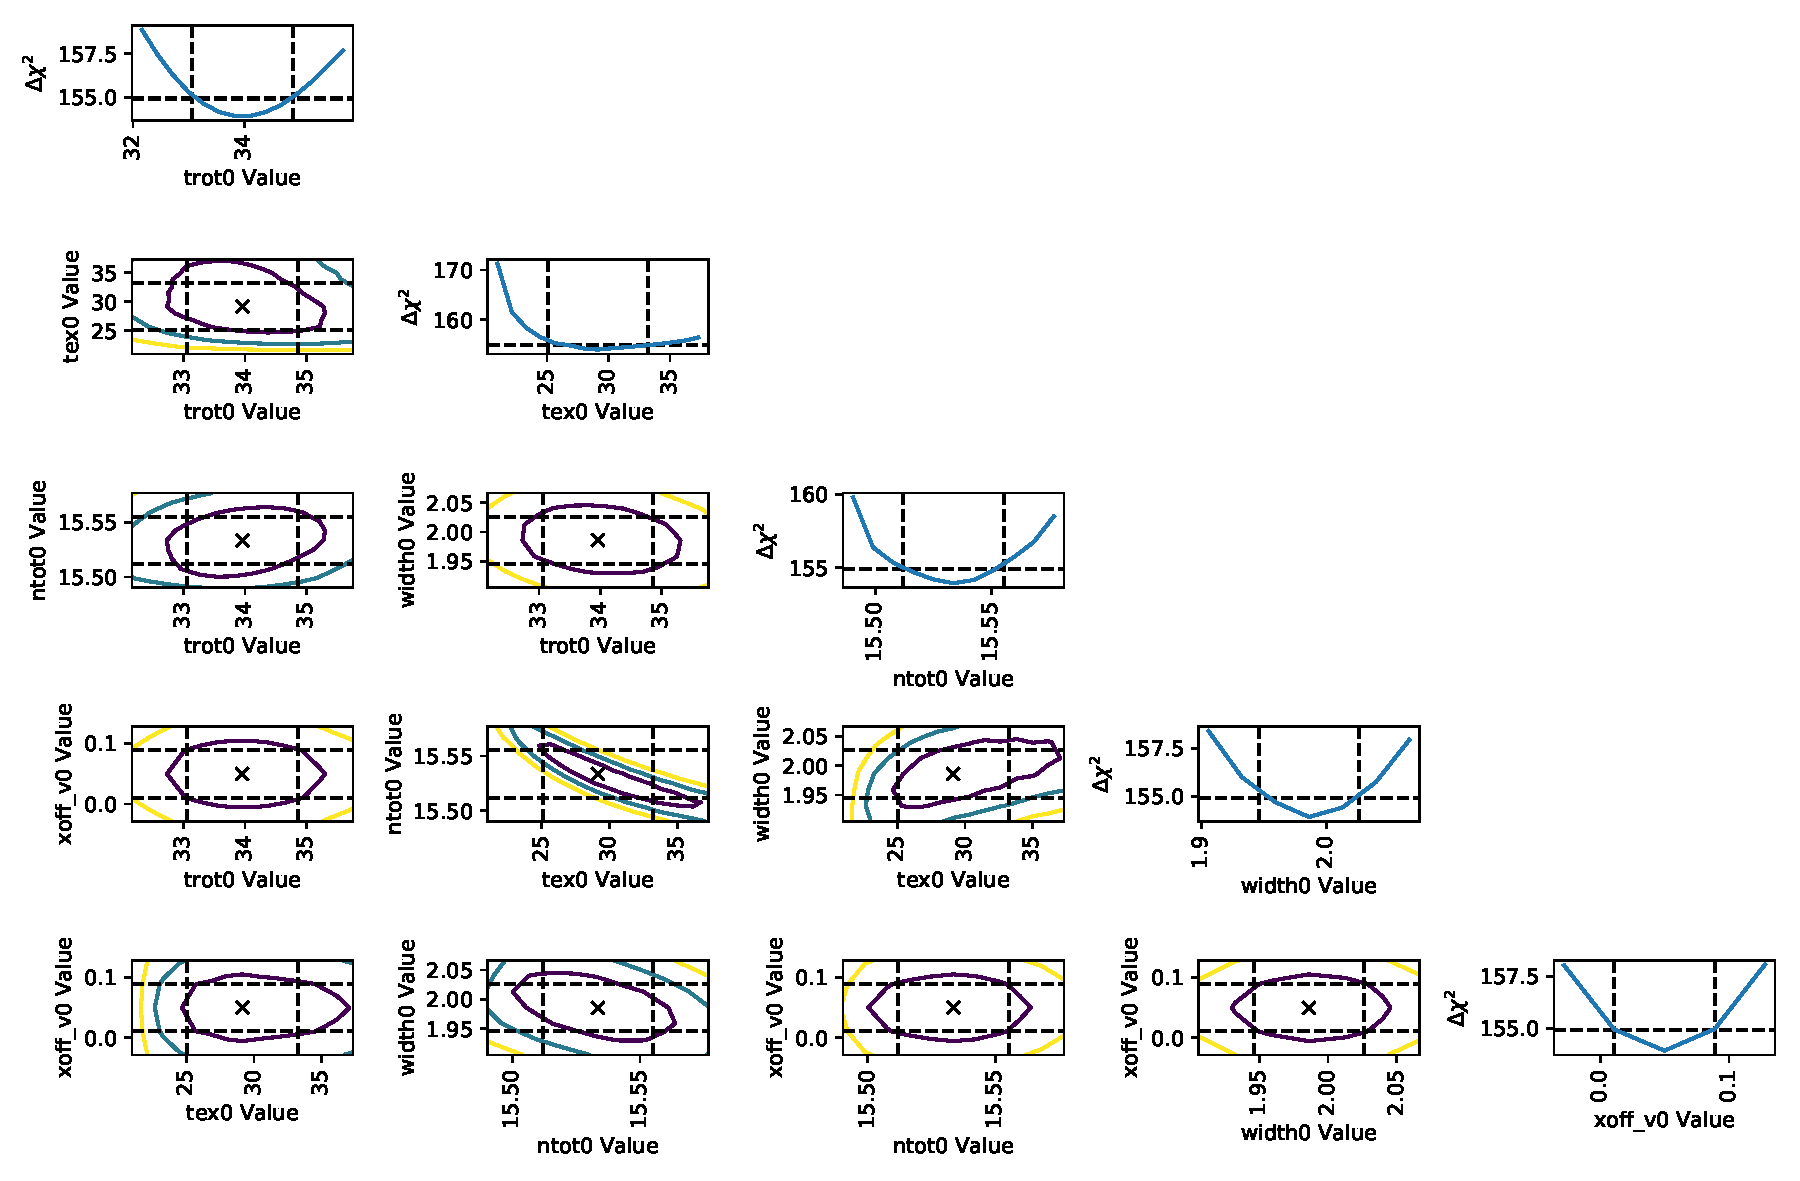
\includegraphics[scale=1,width=7in]{ammonia_LTE_default_error_estimate_demonstration.pdf}
\caption{Error estimate figure for the default \ammonia model.  The panels
are labeled as in Figure \ref{fig:parerrestdemo}.  The most
relevant panel is the ntot0 vs tex0 panel, which plots the column $N$ against
the excitation temperature $T_{\mathrm{ex}}$: both of these parameters govern the peak
amplitude of the spectrum, so they are degenerate.  The vertical dashed lines
do not match the $\Delta\chi^2=1$ positions for $T_{\mathrm{ex}}$ or $N$ partly because
of this degeneracy; the fit errors reported by the Levenberg-Marquardt
algorithm are larger than the directly computed marginal errors. }
\label{fig:nh3parerrestdemo}
\end{figure*}


\section{Comparison of N$_2$H$^+$ (1-0) results with CLASS}
\label{appendix:N2Hp}

One of the most frequently used line transition used to study dense gas kinematics,
in addition to Ammonia, is N$_2$H$^+$ (1-0) at 93.17\,GHz.
The transition displays several hyperfine components with well determined
relative frequencies and weights.
The standard approach is to use the \verb+HFS+ mode within
CLASS.
Here we show that using the already implemented model in \pyspeckit
we obtain the same results in both optically thin and thick models, when
synthetic spectra are created and white noise is added.

The main difference between the CLASS and \pyspeckit parametrization is that
the former does not report excitation temperature ($T_{ex}$), but the area of the
line profile. The reported area is $\tau \times T_{ant}$, where
\begin{equation}
T_{ant}=J(T_{ex}) - J(T_{background})~,
\end{equation}
where
\begin{equation}
J_{\nu}(T) = \frac{h\,\nu}{k_B} \frac{1}{(e^{h\,\nu/k_B\,T} -1)}~.
\end{equation}
We derive the equivalent $T_{ex}$ from the reported line fit parameters.
Moreover, in the optically thin case both fits are performed using the common assumption of
$\tau=0.1$ as a fixed parameter.

Tables \ref{tab:n2hpthin} and \ref{tab:n2hpthick} show the results of fitting
an example spectrum in both CLASS and \pyspeckit.  The resulting fits differ by
$<1\%$ in most parameters, with a slightly greater discrepancy in the velocity
centroid but consistent within the reported fit uncertainties.

%that we speculate is driven by a difference the optimizer's step size
%for that parameter.

\begin{deluxetable}{cccc}
    \label{tab:n2hpthin}
\tablecolumns{4}
\tablecaption{Best fit parameters in optically thin model (3 parameters)\label{table-thin}}
\tablehead{\colhead{Parameter} &\colhead{Input value} & \colhead{pyspeckit fit} & \colhead{CLASS fit}
}
\startdata
%\cutinhead{With all 4 parameters}
%T$_{ex}$      & 9.0    & 5.4$\pm$48 & 2.88430952541\\
%$V_c$          & 0.0    & 0.0001951 &-0.004\\
%$\sigma_v$  & 0.3    & 0.2948$\pm$0.0074 &0.303207\\
%$\tau_{all}$   & 0.01 & 0.026$\pm$0.5 & 0.487 \\
%$Area$ & & & 0.06108\\
%\cutinhead{With 3 parameters}
% 1  6.065E-2(1.164E-3)  2.789E-3(6.844E-3)  0.690   (1.409E-2)  0.100   ( 0.00   )
T$_{ex}$      & 9.0   & 3.454$\pm$0.014     & 3.451\\
$V_c$          & 0.0   & 0.0016              & 0.0028$\pm$0.0068\\
$\sigma_v$  & 0.3   & 0.2942$\pm$0.0062 & 0.2930$\pm$0.0060\\
$\tau_{all}$  & 0.01  & 0.1 & 0.1 \\
$Area$ & & & 0.0607$\pm$0.0012\\
\enddata
\end{deluxetable}


\begin{deluxetable}{cccc}
    \label{tab:n2hpthick}
\tablecolumns{4}
\tablecaption{Best fit parameters in optically thick model (4 parameters)\label{table-thick}}
\tablehead{\colhead{Parameter} &\colhead{Input value} & \colhead{pyspeckit fit} & \colhead{CLASS fit}
}
\startdata
%\cutinhead{With all 4 parameters}
%1   49.0   ( 2.25   )  ********(6.259E-3)  0.716   (1.492E-2)   8.10   (0.590   )
T$_{ex}$     & 9.0  & 9.19$\pm$0.19     & 9.1833\\
$V_c$         & 0.0  & 0.00042 & -0.000$\pm$0.0063\\
$\sigma_v$ & 0.3  & 0.3047$\pm$0.0062 & 0.3041$\pm$0.0063\\
$\tau_{all}$ & 9.0  & 8.13$\pm$0.59   & 8.10$\pm$0.59\\
$Area$ & & & 49.0$\pm$2.25\\
\enddata
\end{deluxetable}

\end{document}
